\chapter{System Overview}
\lhead{\emph{System Overview}}
\label{chapter:system}

The telerobotics system presented in this report consists of a fairly complex image processing pipeline running alongside a simple control system, with little interaction between the two (cf. Figure \ref{fig:system}). The pipeline starts with the two cameras on the rover taking a picture each as close to simultaneously as possible. These images then get abstracted down to edge detected sets of lines, with a set of colours also generated from \emph{Image 1} to combine with its edge detected version later on. These three pieces of data are then compressed into a single packet and transmitted via UDP \cite{postel1980user} to the server. The server splits them up again and produces a depth map from the two edge detected images. This depth map is passed to the 3D Environment to be used to produce a 3D model of the space the cameras were looking at. The server also combines the \emph{Colour Data} and \emph{Edge Detected Image 1} into a full coloured abstraction, which is overlaid onto the 3D model in the 3D environment as a texture. This environment is finally observed in the VR Headset.

The rover is controlled from an Xbox 360 controller \cite{360pad} that is connected to the server. Control inputs for driving the rover, gimble orientation, and parameters for the data abstraction (the only crossover between the control and image processing components) are transmitted to the rover at a fixed rate over UDP. It should be noted that in this system there is no connection between the orientation of the headset and gimble. The focus of this project was on providing the image processing foundations for future high presence systems, therefore the control system is the minimum required to explore the effectiveness of the chosen approach.

\begin{figure}[H]
    \begin{center}
      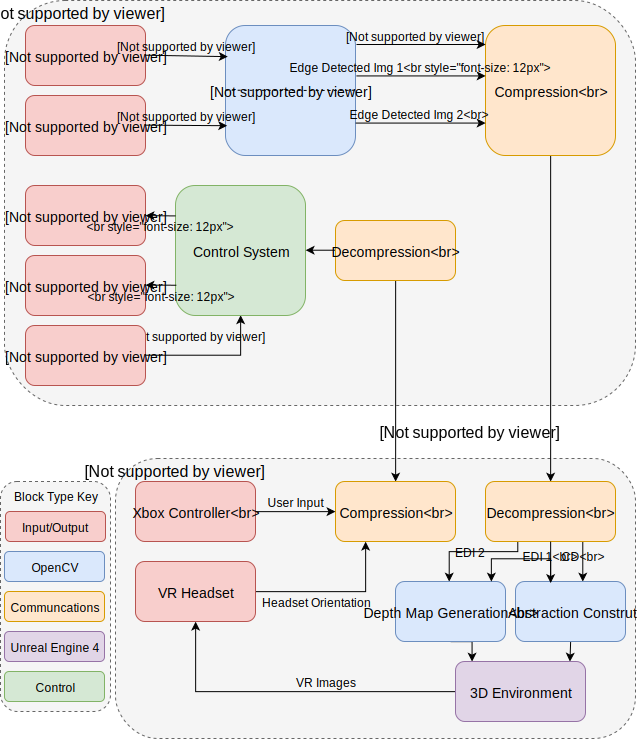
\includegraphics[width=0.8\textwidth]{Figures/System.jpg}
      \caption[System Overview Block Diagram]{System Overview Block Diagram. The red blocks represent input/output, the blue blocks represent image processing steps, the yellow blocks represent communications, and the purple block represents the 3D environment.}
      \label{fig:system}
    \end{center}
\end{figure}